\documentclass{article}[18pt]
\usepackage[dvipsnames]{xcolor}
\usepackage[utf8]{inputenc}
\usepackage[margin=0.7in]{geometry}
\usepackage{parselines} 
\usepackage{amsmath}
\usepackage{amssymb}
\usepackage{titlesec}
\usepackage{pgfplots}
\usepackage{tabularx}

\usepgfplotslibrary{fillbetween}
\usepackage{graphicx}
\usepackage[english]{babel}
\usepackage{fancyhdr}
\usepackage{gensymb}
\usepackage{relsize}
\pgfplotsset{width=10cm,compat=1.9}
\usepackage[super]{nth}
\titlespacing\section{0pt}{14pt plus 4pt minus 2pt}{0pt plus 2pt minus 2pt}
\newlength\tindent
\setlength{\tindent}{\parindent}
\setlength{\parindent}{0pt}
\renewcommand{\indent}{\hspace*{\tindent}}

\pagestyle{fancy}
\fancyhf{}
\rhead{Sam Robbins 13SE}
\lhead{A Level Maths - FP2}
\rfoot{Page \thepage}

\usepackage{cancel}


\setcounter{secnumdepth}{4}
\titleformat{\paragraph}
{\normalfont\normalsize\bfseries}{\theparagraph}{1em}{}
\titlespacing*{\paragraph}
{0pt}{3.25ex plus 1ex minus .2ex}{1.5ex plus .2ex}
\titlespacing\section{0pt}{12pt plus 4pt minus 2pt}{5pt plus 2pt minus 2pt}
\titlespacing\subsection{0pt}{12pt plus 4pt minus 2pt}{5pt plus 2pt minus 2pt}
\titlespacing\subsubsection{0pt}{12pt plus 4pt minus 2pt}{5pt plus 2pt minus 2pt}


\begin{document}
\begin{center}
\underline{\huge Further Complex Numbers}
\end{center}
\section{Expressions of complex numbers}
\subsection{$\mathbf{x+iy}$}
This expresses the coordinate of the point at the end of the vector on the argand diagram.
\\
\begin{center}

\begin{tikzpicture}[scale=0.6]
\begin{axis}[axis lines=middle,ymin=-2.5,ymax=2.5,xmin=-2.5,xmax=2.5,
xtick={-2},xticklabels={$\sqrt{3}$},ytick={1},yticklabels={1},ytick pos=right]
\pgfplotsset{every tick label/.append style={font=\Large}}

\addplot coordinates { (0,0) (-2,1) };
\addplot [dashed] coordinates { (-2,0) (-2,1) };
\addplot [dashed] coordinates { (0,1) (-2,1) };
\end{axis}
\end{tikzpicture}

\end{center}
\subsection{$\mathbf{r(\cos\theta+i\sin\theta)}$}
This expresses the length of the line and the angle anticlockwise from the positive x axis
\begin{center}

\begin{tikzpicture}[scale=0.6]
\begin{axis}[axis lines=middle,ymin=-2.5,ymax=2.5,xmin=-2.5,xmax=2.5,ticks=none]
\pgfplotsset{every tick label/.append style={font=\Large}}

\addplot coordinates { (0,0) (-2,1) };
\draw (axis cs: 0.7,0) arc[radius=80, start angle= 0, end angle= 150];
    \node[] at (axis cs: 0.7,0.7) {$\mathlarger{\frac{5\pi}{6}}$};
\node[blue] at (axis cs: -0.9,0.7) {$\mathlarger{2}$};

\end{axis}
\end{tikzpicture}
\end{center}
$$2\Bigg(\cos\Big(\frac{5\pi}{6}\Big)+i\sin\Big(\frac{5\pi}{6}\Big)\Bigg)$$
\subsection{$re^{i\theta}$}
This uses the same parameters as $r(\cos\theta+i\sin\theta)$
\newpage
\section{Multiplying and dividing complex numbers}
\subsection{Multiplying}
\subsubsection{Trigonometric form}
$$Z_1Z_2=r_1(\cos\theta_1+i\sin\theta_1)\times r_2(\cos\theta_2+i\sin\theta_2)$$
$$=r_1r_2(\cos\theta_1\cos\theta_2-\sin\theta_1\sin\theta_2+i\cos\theta_1\sin\theta_2+i\sin\theta_1\cos\theta_2)$$
Apply the cos addition formula to the first two terms
$$=r_1r_2(\cos(\theta_1+\theta_2)+i\cos\theta_1\sin\theta_2+i\sin\theta_1\cos\theta_2)$$
Apply the sin addition formula to the last two terms
$$=r_1r_2(\cos(\theta_1+\theta_2)+\sin(\theta_1+\theta_2))$$
\subsubsection{Exponential form}
$$\mathlarger{Z_1Z_2=r_1e^{i\theta_1}\times r_2e^{i\theta_2}}$$
Apply laws of indices 
$$\mathlarger{Z_1Z_2=r_1r_2e^{i(\theta_1+\theta_2)}}$$
\subsection{Dividing}
\subsubsection{Trigonometric form}
$$\frac{Z_1}{Z_2}=\frac{r_1(\cos\theta_1+i\sin\theta_1)}{r_2(\cos\theta_2+i\sin\theta_2)}$$
Multiply by the complex conjugate 
$$\frac{Z_1}{Z_2}=\frac{r_1(\cos\theta_1+i\sin\theta_1)}{r_2(\cos\theta_2+i\sin\theta_2)}\times\frac{\cos\theta_2-i\sin\theta_2}{\cos\theta_2-i\sin\theta_2}$$
Expand
$$\frac{Z_1}{Z_2}=\frac{r_1}{r_2}\times\frac{cos\theta_1\cos\theta_2-i\cos\theta_1\sin\theta_2+i\sin\theta_1\cos\theta_2+\sin\theta_1\sin\theta_2}{\cos^2\theta_2-i\cos\theta_2\sin\theta_2+i\sin\theta_2\cos\theta_2+\sin^2\theta_2}$$
Simplify
$$\frac{Z_1}{Z_2}=\frac{r_1}{r_2}\times\Big(\cos(\theta_1-\theta_2)+i\sin(\theta_1-\theta_2)\Big)$$
\subsubsection{Exponential form}
$$\mathlarger{\frac{Z_1}{Z_2}=\frac{r_1}{r_2}\times\frac{e^{i\theta_1}}{e^{i\theta_2}}}$$
$$\mathlarger{\frac{Z_1}{Z_2}=\frac{r_1}{r_2}\times e^{i(\theta_1-\theta_2)}}$$
\subsection{Comparison}
\begin{tabularx}{\textwidth}{|X|X|}
\hline
Multiplying&Dividing\\
\hline	
Multiply modulus, add arguments&Divide modulus, subtract arguments\\
\hline
\end{tabularx}
\newpage
\section{De Moivre's Theorem}
\textcolor{red}{$$\mathlarger{[r(\cos\theta+i\sin\theta)]^n=r^n(\cos(n\theta)+i\sin(n\theta))}$$}
\subsection{Positive proof}
Prove true for n=1
$$r(\cos\theta+i\sin\theta)=r(\cos\theta+i\sin\theta)$$
\begin{center}
True for n=1
\end{center}
Assume true for n=k
$$\mathlarger{[r(\cos\theta+i\sin\theta)]^k=r^k(\cos(k\theta)+i\sin(k\theta))}$$
Prove true for n=k+1
$$[r(\cos\theta+i\sin\theta)]^{k+1}$$
$$[r(\cos\theta+i\sin\theta)]^k\times(r(\cos\theta+i\sin\theta))^1$$
$$r^k(\cos(k\theta)+i\sin(k\theta))\times r(\cos\theta+i\sin\theta)$$
$$r^kr(\cos(k\theta+\theta)+i\sin(k\theta+\theta))$$
$$r^{k+1}(\cos((k+1)\theta)+i\sin((k+1)\theta))$$
True
\subsection{Negative proof}
n=-m
$$[r(\cos\theta+i\sin\theta)]^{-m}$$
Multiply by complex conjugate
$$\frac{1}{[r(\cos\theta+i\sin\theta)]^m}\times\frac{[r(\cos\theta-i\sin\theta)]^m}{[r(\cos\theta-i\sin\theta)]^m}$$
Apply positive De Moivre's Theorem
$$\mathlarger{\frac{r^m(\cos(m\theta)-i\sin(m\theta))}{r^m(\cos(m\theta)+i\sin(m\theta))\times r^m(\cos(m\theta)-i\sin(m\theta))}}$$
Simplify and expand
$$\mathlarger{\frac{\cos(m\theta)-i\sin(m\theta)}{r^m(\cos^2m\theta-i\cos m\theta\sin m\theta+i\cos m\theta\sin m\theta+\sin^2m\theta}}$$
Simplify
$$\frac{\cos m\theta-i\sin m\theta}{r^m}=r^{-m}(\cos m\theta-i\sin m\theta)$$
Rewrite
$$r^{-m}(\cos(-m\theta)+i\sin(-m\theta))$$
Replace -m with n
$$r^n(\cos(n\theta)+i\sin(n\theta))$$
\newpage
\subsection{Applying De Moivres' Theorem}
We can use the binomial expansion along with De Moivre's theorem to rewrite trigonometric expressions. This can be useful when integrating etc.
\subsubsection{Example 1}
\textit{Rewrite $\cos5\theta$ in powers of $\cos\theta$}
$$(\cos\theta+i\sin\theta)^5$$
Apply DM theorem
$$\cos5\theta+i\sin5\theta$$
Apply the binomial expansion to the initial expression
$$\cos^5\theta+5\cos^4\theta i\sin\theta+10\cos^3\theta(i\sin\theta)^2+10\cos^2\theta(i\sin\theta)^3+5\cos\theta(i\sin\theta)^4+(i\sin\theta)^5$$
Simplify
$$\cos^5\theta+5i\cos^4\theta\sin\theta-10\cos^3\theta\sin^2\theta-10i\cos^2\theta\sin^3\theta+5\cos\theta\sin^4\theta+i\sin^5\theta$$
Equate the real parts of this to the real parts of the result from DM theorem
$$\cos5\theta=\cos^5\theta-10\cos^3\theta\sin^2\theta+5\cos\theta\sin^4\theta$$
Replace sin terms with cos
$$\cos5\theta=\cos^5\theta-10\cos^3\theta(1-\cos^2\theta)+5\cos\theta(1-\cos^2\theta)^2$$
Simplify
$$\cos5\theta=\cos^5\theta-10\cos^3\theta+10\cos^5\theta+5\cos\theta(1-\cos\cos^2\theta+cos^4\theta)$$
Simplify further
$$\cos5\theta=\cos^5\theta-10\cos^3\theta+10\cos^5\theta+5\cos\theta-10\cos63\theta+5\cos^5\theta$$
Collect terms
$$\cos5\theta=16\cos^5\theta-20\cos^3\theta+5\cos\theta$$
\newpage
\subsubsection{Z formulas}
If $z=\cos\theta+i\sin\theta$
$$z+\frac{1}{z}=2\cos\theta$$
$$z-\frac{1}{z}=2i\sin\theta$$
$$z^n+\frac{1}{z^n}=2\cos n\theta$$
$$z^n-\frac{1}{z^n}=2i\sin n\theta$$
\paragraph{Example}
\textit{Express $\cos^5\theta$ in the form $a\cos5\theta+b\cos3\theta+c\cos\theta$}
Create the situation using the z formulas
$$\Bigg(z+\frac{1}{z}\Bigg)^5=(2\cos\theta)^5=32\cos^5\theta$$ 
Expand using the binomial
$$\textcolor{red}{z^5}+\textcolor{Green}{5z^4\times\frac{1}{z}}+\textcolor{Plum}{10z^3\times\frac{1}{z^2}}+\textcolor{Plum}{10z^2\times\frac{1}{z^3}}+\textcolor{Green}{5z\times\frac{1}{z^4}}+\textcolor{red}{\frac{1}{z^5}}$$
Combine like coloured term using z formula
$$32\cos^5\theta=\textcolor{red}{2\cos\theta}+\textcolor{Green}{10\cos3\theta}+\textcolor{Plum}{20\cos\theta}$$
$$\cos^5\theta=\frac{\cos\theta}{16}+\frac{5\cos3\theta}{16}+\frac{5\cos\theta}{8}$$
\section{Solving complex equations}
For any complex number, we generally define the argument to be between $-\pi$ and $\pi$. However we can add multiples of $2\pi$ to the argument to get equivalent answers.\\
\\
We shall use this fact to find all solutions to complex equations.\\
\\
Note: The number of solutions is equal to the order of the equation.
\subsection{Example}
\textit{Solve:}\\
$z^5=i$
$$r=1 \quad \theta=\frac{\theta}{2}$$
$$z^5=\cos(\frac{\pi}{2}+2k\pi)+i\sin(\frac{\pi}{2}+2k\pi)$$
$$z=\cos\Bigg(\frac{\frac{\pi}{2}+2k\pi}{5}
\Bigg)+i\sin\Bigg(\frac{\frac{\pi}{2}+2k\pi}{5}\Bigg)$$
5 Solutions: k=-2,-1,0,1,2\\
$k=-2 \quad z=-0.588-0.809i$\\
$k=-1 \quad z=0.588-0.809i$\\
$k=0 \quad z=0.951+0.309i$\\
$k=1 \quad z=i$\\
$k=2 \quad z=-0.951+0.309i$
\newpage
\section{Loci on the complex plane}
\subsection{Lines}
\subsubsection{$\mathbf{|z-z_1|=r}$}
$|z-z_1|=r$ is represented by a circle, centre $(x_1,y_1)$ with a radius r, where $z_1=x_1+iy_1$.\\
\\
This is the same as the Cartesian equation:
$$(x-x_1)^2+(y-y_1)^2=r^2$$
This looks like the graph:\\
\begin{tikzpicture}[scale=0.8]
\begin{axis}[axis lines=middle,ymin=-5,ymax=5,xmin=-5,xmax=5,ticks=none]
\pgfplotsset{every tick label/.append style={font=\Large}}

\draw (axis cs:1,2) circle [black, radius=3];
    \node[] at (axis cs: 1,2) {$(x_1,y_1)$};
    \node[] at (axis cs: 2,3.3) {$r$};
    
           \node[anchor=west] (source) at (axis cs:1,2){};
       \node (destination) at (axis cs:3,4.5){};
       \draw[->](source)--(destination);
\end{axis}
\end{tikzpicture}
\subsubsection{$\mathbf{|z-z_1|=|z-z_2|}$}
$|z-z_1|=|z-z_2|$ is represented by a perpendicular bisector of the line segment joining points $z_1$ and $z_2$\\
\\
To find the Cartesian form, replace z with $x+iy$ and expand, squaring both sides to remove the modulus signs.\\
\\
This looks like the graph:\\
\begin{tikzpicture}[scale=0.8]
\begin{axis}[axis lines=middle,ymin=-5,ymax=5,xmin=-5,xmax=5,ticks=none]
\pgfplotsset{every tick label/.append style={font=\Large}}

    \node[] at (axis cs: 1,3) {$z_2$};
    \node[] at (axis cs: 3,1) {$z_1$};
\addplot coordinates { (-4,-4) (4,4) };    
    
\end{axis}
\end{tikzpicture}\\
For cases where there is a constant in front of one of the modulus signs, use the algebraic method to find the Cartesian form, then plot that.
\newpage
\subsubsection{$\mathbf{\arg(z-z_1)=\theta}$}
$\arg(z-z_1)=\theta$ is represented by the half-line from the fixed point $z_1$, making an angle $\theta$ with a line from the fixed point $z_1$, parallel to the real axis.\\
\\
To find the Cartesian form, replace z with $x+iy$ and separate into the real and imaginary parts. Then use the trigonometric identity $\tan\theta=\dfrac{\textrm{Opposite}}{\textrm{Adjacent}}$ and simplify.\\
\\
When plotting remember that $\theta$ is the angle anticlockwise.\\
\begin{tikzpicture}[scale=0.8]
\begin{axis}[axis lines=middle,ymin=-2.5,ymax=2.5,xmin=-2.5,xmax=2.5,ticks=none]
\pgfplotsset{every tick label/.append style={font=\Large}}

\addplot coordinates { (0,0) (-2,1) };
\draw (axis cs: 0.7,0) arc[radius=80, start angle= 0, end angle= 150];
    \node[] at (axis cs: 0.7,0.7) {\Large $\theta$};
\node[blue] at (axis cs: -2,1.2) {\LARGE $z_1$};

\end{axis}
\end{tikzpicture}
\subsubsection{$\mathlarger{\mathbf{\arg\Big(\frac{z-z_1}{z-z_2}\Big)}}$}
$\mathlarger{\arg\Big(\frac{z-z_1}{z-z_2}\Big)}$ represents an arc anticlockwise between $z_1$ and $z_2$
\subsection{Regions}
\subsubsection{$\mathbf{|z-(2+3i)|\leqslant3}$}
This is the area inside the circle represented by $|z-(2+3i)|\leqslant3$\\
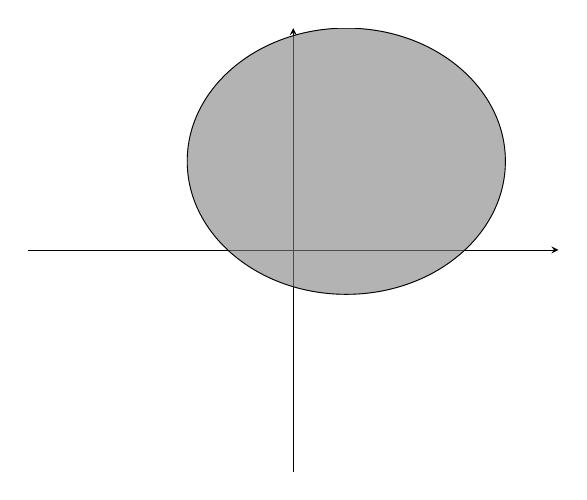
\begin{tikzpicture}[scale=0.8]
\begin{axis}[axis lines=middle,ymin=-5,ymax=5,xmin=-5,xmax=5,ticks=none]
\pgfplotsset{every tick label/.append style={font=\Large}}

\filldraw[gray,opacity=0.6] (axis cs:1,2) circle [black, radius=3];
\draw (axis cs:1,2) circle [black, radius=3];
\end{axis}
\end{tikzpicture}
\newpage
\subsubsection{$\mathbf{|z-3|<|z-5|}$}
This is the area to one side of the perpendicular bisector represented equal to $|z-3|=|z-5|$\\
\pgfplotsset{compat=newest}

\begin{tikzpicture}[scale=0.8]
\begin{axis}[axis lines=middle,ymin=-5,ymax=5,xmin=-5,xmax=5,xtick={3,4,5}, ytick={0},ytick pos=right]
\addplot coordinates { (4,-5) (4,5) };
\filldraw [gray,opacity=0.6] (-5,-5) rectangle (4,5);
\end{axis}
\end{tikzpicture}
\subsubsection{$\mathbf{0\leqslant\arg(z-2)<\frac{\pi}{4}}$}
This is the area between the positive real axis and the half line equal to $\arg(z-2)=\frac{\pi}{4}$\\
\begin{tikzpicture}[scale=0.8]
\begin{axis}[axis lines=middle,ymin=-5,ymax=5,xmin=-5,xmax=5,xtick={2}, ytick={0},ytick pos=right]
\addplot coordinates { (2,0) (5,3) };
\filldraw[gray,opacity=0.6] (2,0) -- (5,0) -- (5,3) -- cycle;

\end{axis}
\end{tikzpicture}
\end{document}